% Model Inversion Attacks that Exploit Confidence Information and Basic Countermeasures (Frederickson)
%Algorithms that remember: model inversion attacks and data protection law
\section{Grundlegende Konzepte und Modelle}\label{chpt:Stand_der_Technik_MI}
%Vorstellung grundlegender Konzepte und Modelle im Zusammenhang mit Model Inversion Attacks.
Mit stetigem Wandel und Weiterentwicklung digitaler Systeme gewinnt die Sicherheit und Robustheit zunehmend an Bedeutung. Insbesondere mit der vermehrten Integration von Künstlicher Intelligenz (KI) ergeben sich neue Herausforderungen im Kontext der Sicherheits- und Robustheitsaspekte. Dieses Unterkapitel widmet sich den grundlegenden Aspekten des Modell-Inversionsangriffs, einem Schlüsselelement in der Diskussion um die Robustheit neuronaler Netzwerke.

Die fundamentale Idee dieses Angriffsszenarios manifestiert sich durch die Rekonstruktion von im Trainingsprozess verwendeten Datenpunkten, wodurch die Privatsphäre einzelner Individuen des Trainingsdatensatzes kompromittiert wird. Dabei geht es um den gezielten Versuch, sensible Informationen durch eine geschickte Interaktion mit dem Modell zu extrahieren und somit die Integrität der Trainingsdaten zu durchbrechen (siehe \ref{subsec: MIAttack}). 

Die Durchführung einer Modell-Inversionsattacke kann basierend auf unterschiedlichen Modellarchitekturen stattfinden. Das Paper \glqq Privacy in Pharmacogenetics\grqq{} (\cite{fredrikson_privacy_2014}) befasst sich mit der Angriffsdurchführung basierend auf einem \textit{Regressionsmodell} unter anderem im WhiteBox-Setting. Hierbei sind dem Angreifer, der mit dem Ziel der Vorhersage des Genotyps eines bestimmten Individums auf Basis verschiedener Merkmale und Attribute der Person handelt, Modellstrukturen und -parameter, wie auch Attribute der Person bekannt (\cite[20]{fredrikson_privacy_2014}). Das Hauptziel des Angriffs beschreibt die Gewinnung sensibler Informationen, wordurch die Privatsphäre dieser verletzt wird. Mit Hilfe des Algorithmus, der für die Durchführung der Modell-Inversionsattacke programmiert wurde und unabhängig von zugrundeliegenden Modellstrukturen ist, kann durch die Invertierung des Modells auf genetische Marker der Person Rückschluss gezogen werden. Dem Autor zur Folge sei der verallgemeinerte Modellinversionsalgorithmus optimal, da dieser die erwartete Fehlervorhersage des Angreifers minimiert. Zudem sei der Algorithmus nahezu so effektiv wie speziell trainierte Regressionsmodelle, die auf die Vorhersage dieser Marker abzielen. Neben den Modell-Inversionsangriffen werden auch Verteidigungsmechanismen beschrieben, die zur Sicherung der Privatsphäre beitragen kann. Einer der Algorithmen ist die Integration von differentieller Privatsphäre. Das genutzte Regressionsmodell ist auf Basis des IWPC Datensatzes trainiert und wird für die Durchführung und Analyse von Angriffsszenarios, sowie Auswertung der Verteidigungsstrategie verwendet.

Eine weitere Modellarchitektur, die eine Anfälligkeit gegenüber Modell-Inversionsangriffen bietet, sind Entscheidungsbäume (\cite[S. 4 ff.]{fredrikson_model_2015}), welche vom Autor als Modelle beschrieben werden, die den Merkmalsraum in disjunkte Regionen partitioniert und Vorhersagen für Instanzen basierend auf Merkmalen macht. Dabei wird beschrieben, dass zwischen \textit{Klassifikationsbäumen}, deren Zielvariable diskret ist, und Regressionsbäumen, deren Zielvariable kontinuierlich ist, zu unterscheiden ist. In Betracht auf Modell-Inversionsangriffe nutzt der Autor Black- und Whitebox Settings für die Durchführung und Evaluierung der Angriffe. Im BlackBox Setting wird eine angepasste Form des Algoritmus für Regressionsmodelle (\cite[21]{fredrikson_privacy_2014}) verwendet, der auf die Grundarchitektur und der veränderten Ausgabe der Entscheidungsbäume zurückzuführen ist. Das WhiteBox Verfahren dahingegen verwendet Konfizenzwerte, um die sensiblen Informationen zu inferieren, indem es die Konfidenzwerte für verschiedene Klassifikationen analysiert und daraus Rückschlüsse auf mögliche Werte der sensiblen Merkmale zu ziehen. Durch das Kennen der internen Modellstruktur ist es möglich, diese sensiblen Informationen mit hoher Präzision zu inferieren. Besonders für Datenpunkte, die Teil des Trainingsdatensatzes sind. 

Eine wichtige Rolle im Bereich der Inversions-Angriffe spielt die Modellarchitektur der neuronalen Netzwerke zur Klassifikation von Bildern. Diese dienen als Klassifikator für ungesehene Eingaben und eröffnen dem Angreifer die Möglichkeit zur Rekonstruktion der im Training verwendeten Datenpunkte. Das Paper \glqq Model Inversion Attacks that Exploit Confidence Information and Basic Countermeasures\grqq{} (\cite[7]{fredrikson_model_2015}) legt das Augenmerk auf Modelle zur Gesichtsidentifikation und nutzt jeweils ein \textit{Softmax-Regressionsmodell}, \textit{MLP} und \textit{SDAE-Modell} zur Durchführung von Modelinversionsangriffen, wobei alle Architekturen einen vergleichsweise einfachen Aufbau vorweisen. Das Softmax-Regressionsmodell ist mit einer generalisierten Version eines logistischen Regressionsmodell zu beschreiben, wobei die Klassenvariable mehr als 2 Werte annehmen kann. Da der zugrundeliegende Datensatz aus 40 Klassen besteht, kann ein austrainiertes Regressionsmodell zwischen 40 verschiedenen Werten für die Klassenvariable unterscheiden. Der Hauptunterschied zwischen den genannten Modellen  besteht lediglich in der Anzahl verborgener Schichten. Das MLP weist genau eine verborgene Schicht auf, wohingegehen das Softmax-Regressionsmodell keine besitzt. Das SDAE-Modell hingegen weist sogar 2 verborgene, vollvermaschte Schichten, die als \glqq Denoising Autoencoder\grqq{} verwendet werden, auf und ist damit in der Lage Merkmale und Muster in den Eingabedaten zu erfassen. Das Paper befasst sich auf Basis der genannten Modelle mit der Ausführung einer WhiteBox-Modell-Inversionsattacke, die ganze Bilder mit den jeweiligen Pixelwerten versucht zu rekonstruieren. Dies geschieht auf Basis des beschriebenen Algorithmus, der im Paper beschrieben ist (\cite[8]{fredrikson_model_2015}) und den Gradientenabstieg für die Miminierung der Kostenfunktion verwendet. Ziel der Arbeit ist die Untermalung der Gefahr von Modell-Inversionsangriffen auf Basis verschiedener Modellarchitekturen.

Die jeweiligen Erkenntnisse und Ergebnisse der aufgezeigten Forschungsbeiträge werden im Folgekapitel bleuchtet.
\section{Forschungsergebnisse}\label{chpt:MIAttacksResearch}
%Zusammenfassung der wichtigsten Forschungsergebnisse und Erkenntnisse im Bereich Model Inversion Attacks.
Die Ergebnisse der Netzwerke zur Vorhersage von Genotypen (\cite[S. 7 ff.]{fredrikson_privacy_2014}) werden auf Basis des linearen Regressionsmodells durch die Ausführung des im Paper beschriebenen Algorithmus zur Durchführung der Modell-Inversionsattacke bereitgestellt und mit Vorhersagen eines optimalisierten logistischen Regressionsmodell verglichen. Die Qualitätsbewertung des Angriffs erfolgt hierbei zum einen mittels \glqq AUCROC\grqq{} Kurve, sowie auf Basis der Genauigkeit von verschiedenen Modellen und Idealen. Um die Effektivität und Qualität des Angriffs bewerten zu können, nutzt Frederikson eine Vergleichsmethode, welche Algorithmik-Vorhersagen, Ideal-Vorhersagen und BaseLine-Genauigkeit gegenüberstellt. Dabei beschreibt die BaseLine-Genauigkeit diese, welche durch Raten des wahrscheinlichsten Genotyps auf Basis der gegebenen marginalen Priorität, die für die jeweilige Klasse variiert, erzielt wird.
\begin{figure}[H]
	\centering
	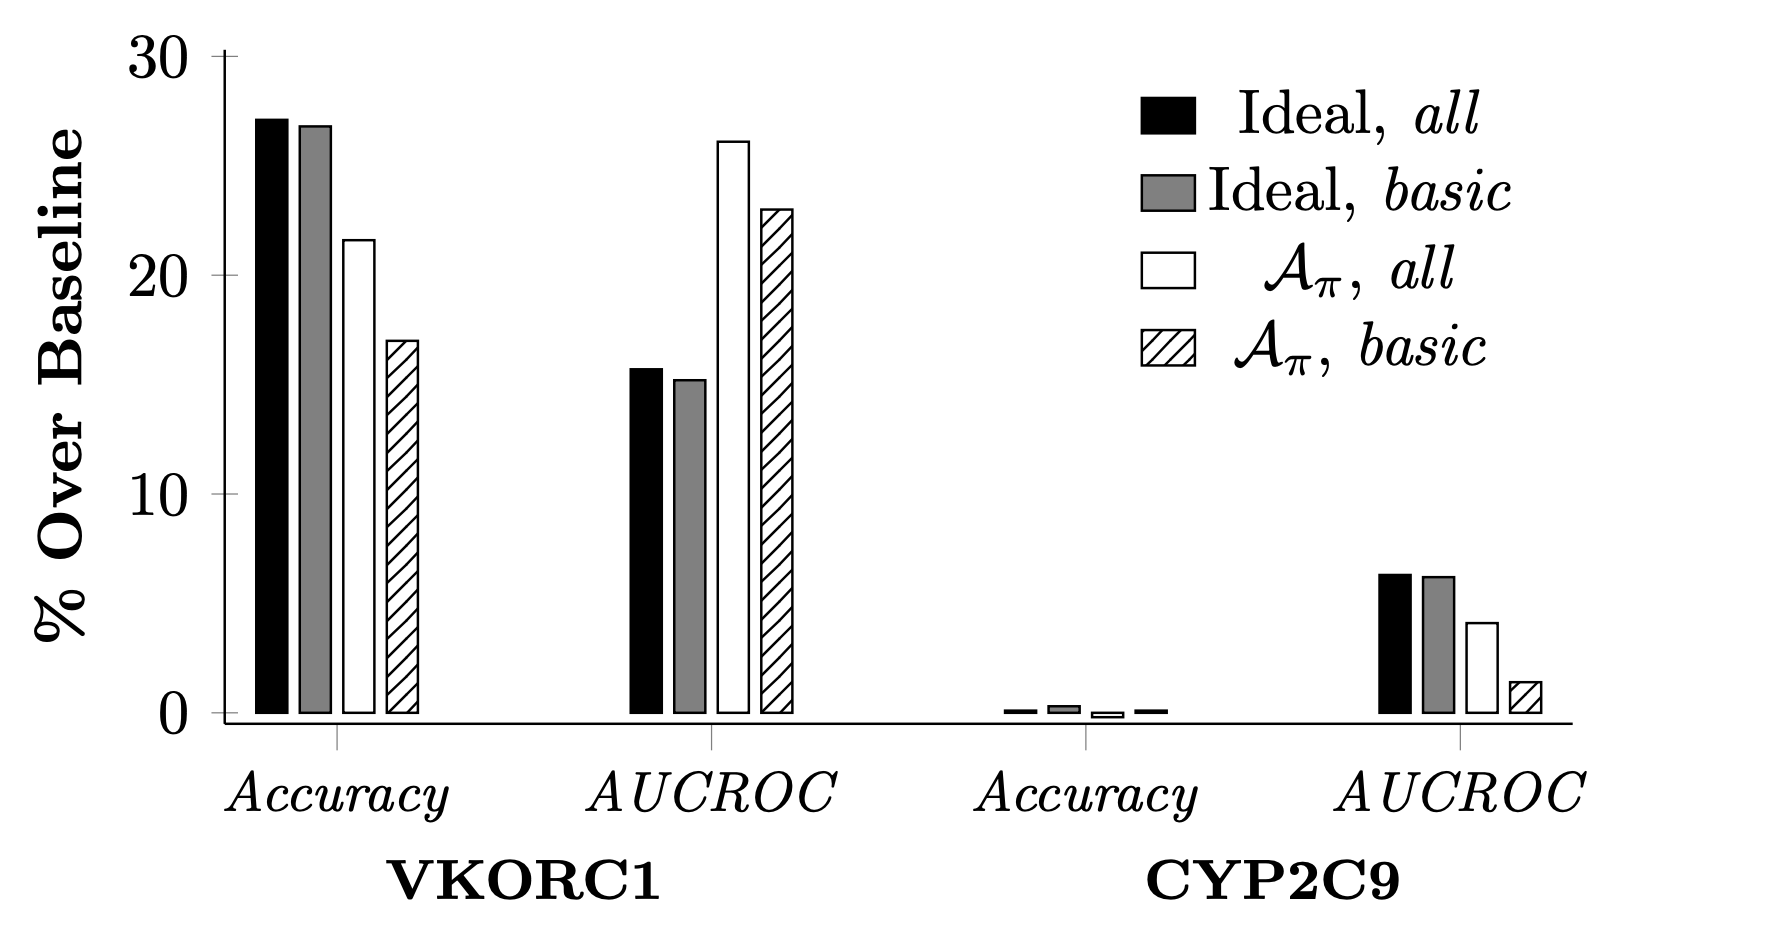
\includegraphics[width=0.6\linewidth]{Bilder/paper_fred_2014_graph.png}
	\caption{Modell-Inversionsangriff Ergebnisse (\cite[S. 7, Figure 3]{fredrikson_privacy_2014})}
	\label{img:frederikson_evaluation}
\end{figure}
Gemäß Abbildung \ref{img:frederikson_evaluation}, entnommen aus dem veröffentlichten Paper von Frederikson, zeigt sich durch die Analyse der AUCROC-Kurve, dass der Algorithmus (Modell-Inversion) in der Lage ist, VKORC1-Genotypen präziser vorherzusagen als das Idealmodell. Dennoch weisen die durch den Algorithmus erzeugten Ergebnisse eine leicht geringere Genauigkeit im Vergleich zu vorab trainierten Idealmodellen auf, weshalb die Leistung des Angriffs geringfügig schlechter ist als die des ursprünglichen Modells.
Im Gegensatz zu VKORC1 kann für CYP2C9 aufgrund der Komplexität und der damit verbundenen Schwierigkeiten bei der Vorhersage weder mit Hilfe des Idealmodells noch des Algorithmus eine annähernd hohe Genauigkeit erreicht werden. Dies führt dazu, dass die Baseline-Genauigkeit deutlich höher ist als andere Genauigkeiten, und die Effizienz des Angriffs bei CYP2C9 im Vergleich zu VKORC1-Genotypen erheblich schlechter ist.
Nach der Durchführung wurde zudem die Genauigkeit der Modelle im Hinblick auf Trainings- und Validierungsgenauigkeit überprüft, wobei eine deutliche Verschlechterung im Bezug auf ungesehene Validierungsdaten festgestellt worden war.

Auf Basis der in Kapitel \ref{chpt:Stand_der_Technik_MI} dargestellten Entscheidungsbäumen wurden verschiedene Experimente durchgeführt, mit dem Ziel der Modell-Inversionsdemonstration. Der zugrunde liegende Datensatz ist dabei zum einen der \glqq Five-Thirty-Eight\grqq{}-Datensatz, welcher durch Umfragen erworben wurde und verschiedene Merkmale, wie demografische Informationen und Vorlieben, enthält. Zudem wurde der \glqq GSS marital happiness\grqq{}-Datensatz verwendet, der verschiedene Aspekte des Eheglücks beinhaltet. Zu den Mermalen gehören hierbei neben demografischen Informationen auch Interessen und Einstellungen von US-amerikanischen Einwohnern. Mit diesen Datensätzen als Grundlage wird versucht, sensible Informationen anhand Modell-Inversionsangriffen aus den Daten zu extrahieren. Die Angriffe, basierend auf spezifischen Algorithmen, wurde sowohl im WhiteBox- sowie im BlackBox-Setting für jede einzelne Zeile des Datensatzes durchgeführt. Die zugrunde liegenden Modelle wurden von \glqq Online-Anbietern\grqq{} bezogen, um das Risiko öffentlich verfügbarer Modelle zu bewerten. In der Auswertung (siehe Bild \ref{img:frederikson_2015_evaluation}) verschiedener Durchführungen (\cite[S. 5 ff.]{fredrikson_model_2015}) wird zum einen beschrieben, dass auf WhiteBox-basierte Inversionsangriffe eine hohe Präzision bezüglich positiver Instanzen der sensiblen Variablen zu erkennen ist. Somit kann ein Angreifer, der Zugriff auf das zugrundeliegende Modell besitzt, verhältnismäßig einfach sensible Informationen, wie \glqq Ja\grqq{}-Antworten auf bestimmte Fragen, extrahieren. Das Risiko der \glqq ungewollten Bereitstellung\grqq{} sensibler Informationen ist deutlich höher, wenn der Repräsentant Teil des Trainingsdatensatzes ist und dabei effektiv verwendet wurde. 
\begin{figure}[H]
	\centering
	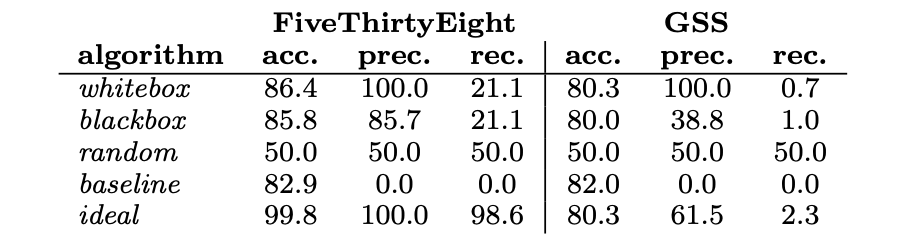
\includegraphics[width=0.6\linewidth]{Bilder/frederikson_2015_1.png}
	\caption{MI-Ergebnisse für BigML-Modelle (\cite[S. 6, Figure 4]{fredrikson_model_2015})}
	\label{img:frederikson_2015_evaluation}
\end{figure}
Anhand der in Abbildung \ref{img:frederikson_2015_evaluation} dargestellten Angriffsergebnisse lässt sich erkennen, dass die Leistung des WhiteBox-Verfahrens, das keine falsch-positiven Ausgaben produziert, deutlich höher ist, als die des BlackBox-Verfahren. Verdeutlicht wird, dass beide Angriffe die Genauigkeit der Zufallsgenerierung übertreffen, kein Angriff aber einen höhere Recall aufgrund der verzerrten Verteilung des sensiblen Mermals erreichen konnte. In einer weiteren Abbildung (\cite[S. 7, Figure 5]{fredrikson_model_2015}) wird ein Vergleich zwischen Angriffsdurchführungen von Trainings- und Testdaten dargestellt, womit ein erhebliches Risiko für die Vertraulichkeit durch den Einbezug von Daten in den Trainingsprozess verdeutlicht wird. 

Die beiden Angriffe bezüglich der in Kapitel \ref{chpt:DefenseMI} dargestellten Modelle (\cite[S. 7 ff.]{fredrikson_model_2015}) zur Gesichtserkennung setzen voraus, dass der Angreifer nur Zugriff auf das jeweilig trainierte Modell hat, Trainingsdaten, die ursprünglich verwendet wurden, jedoch unbekannt sind. Dabei werden zwei Arten von Modell-Inversionsangriffen ausgeführt. Im ersten Angriff handelt es sich um ein Szenario in welchem der Angreifer das Label beziehungsweise einen eindeutigen Indikator für eine bestimmte Person kennt, um diese rekonstruieren zu können. Dabei kennt der Angreifer neben dem Ziel-Label keine weiteren Parameter und Strukturen. Mit Hilfe des im Paper definierten Angriffsalgorithmus (MI-Face) werden Bilder generiert, die mit Hilfe der Nachbearbeitungsfunktion (Process) qualitativ verbessert werden können. Bei der Verwendung des SDAE-Modells verwendet der Autor eine abgeänderte Process-Funktion (Process-DAE), um Kandidatenlösungen im latenten Raum der ersten Autoencoder-Schicht zu generieren. Diese Funktion dekodiert während jeder Iteration den kandidaten in den ursprünglichen Pixelraum, wendet einen Entrauschungsfilter gefolgt von einem Schärfefilter an und kodiert die resultierenden Pixel in den latenten Raum zurück. Dadurch wird viel Rauschen aus der finalen Rekonstruktion entfernt. 
\begin{figure}[H]
	\centering
	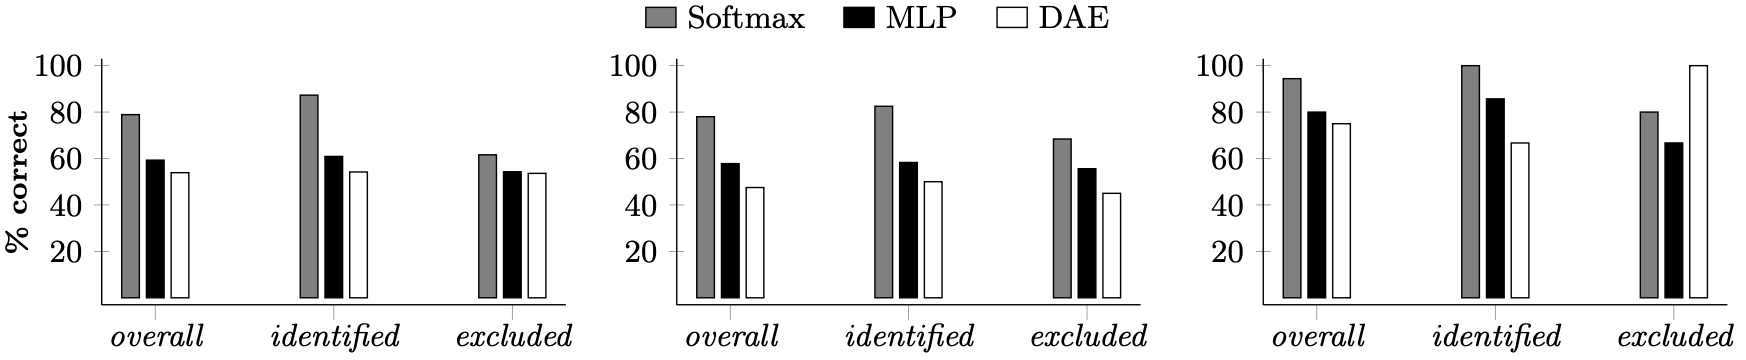
\includegraphics[width=1\linewidth]{Bilder/frederikson_2015_2.png}
	\caption{MI-Ergebnisse des \glqq Mechanical Turk Survey\grqq{} (\cite[S. 10, Figure 9]{fredrikson_model_2015})}
	\label{img:frederikson_2015_evaluation2}
\end{figure}
Die in Abbildung \ref{img:frederikson_2015_evaluation2} dargestellten Grafiken entstanden auf Basis eines bestimmten Experimentier- und Evaluierungskonzept, wobei Mechanical Turk-Arbeiter gebeten wurden, ein rekonstruiertes Bild einem von fünf Gesichtsbildern des AT\&T-Datensatzes zuzuordnen. Falls dieser der Meinung war, die Generierung würde keinem der gezeigten Bilder entsprechen, war dies auch eine mögliche Antwort. Dabei wurde jeder Satz der Experimente mit den selben Testbildern drei mal durchgeführt, um die Konsistenz der Arbeiterantworten zu untersuchen. Alle dem Turk-Arbeiter gezeigten Bilder entstammten aus dem Validierungsdatensatz, weshalb sie kein Teil des Trainingsdatensatzes waren. Durch verdeutlichung der Grafik im vorerst die Begrifferklärungen des Autors: \textit{overall} beschreibt das Ergebnis, wobei der Arbeiter alle Antworten korrekt gegeben hat. \textit{Identified} bezieht sich auf diejenigen Fälle, bei denen die Arbeiter die richtige Person, wenn diese Teil der Testbilder war, identifizieren konnte. \textit{Excluded} sind genau die Fälle, in denen Personenbilder der angegriffenen Label nicht angezeigt wurde und der Arbeiter korrekterweise kein Bild zugeordnet hat.
Der linke Plot aus Abbildung \ref{img:frederikson_2015_evaluation2} stellt die Ergebnisse über alle Antworten gemittelt da. Der mittlere Plot dahingegen visualisiert die Ergebnisse, bei denen mindestens zwei der drei Antworten korrekt waren. Der rechte Plot visualisiert die Ergebnisse geschulter Arbeiter, die sich durch mindestens fünf abgeschlossene Aufgaben mit einer Genauigkeit von 75\% oder mehr auszeichnen.
Mit Hilfe der Ergebnisdarstellungen lässt sich erkennen, dass Modell-Inversionsangriffe bezüglich des Softmax-Regressionsmodells am besten erraten wurden, wodurch man auf die genauste und qualitativ beste Repräsentation der Generierungen schließen kann. 
\begin{figure}[H]
	\centering
	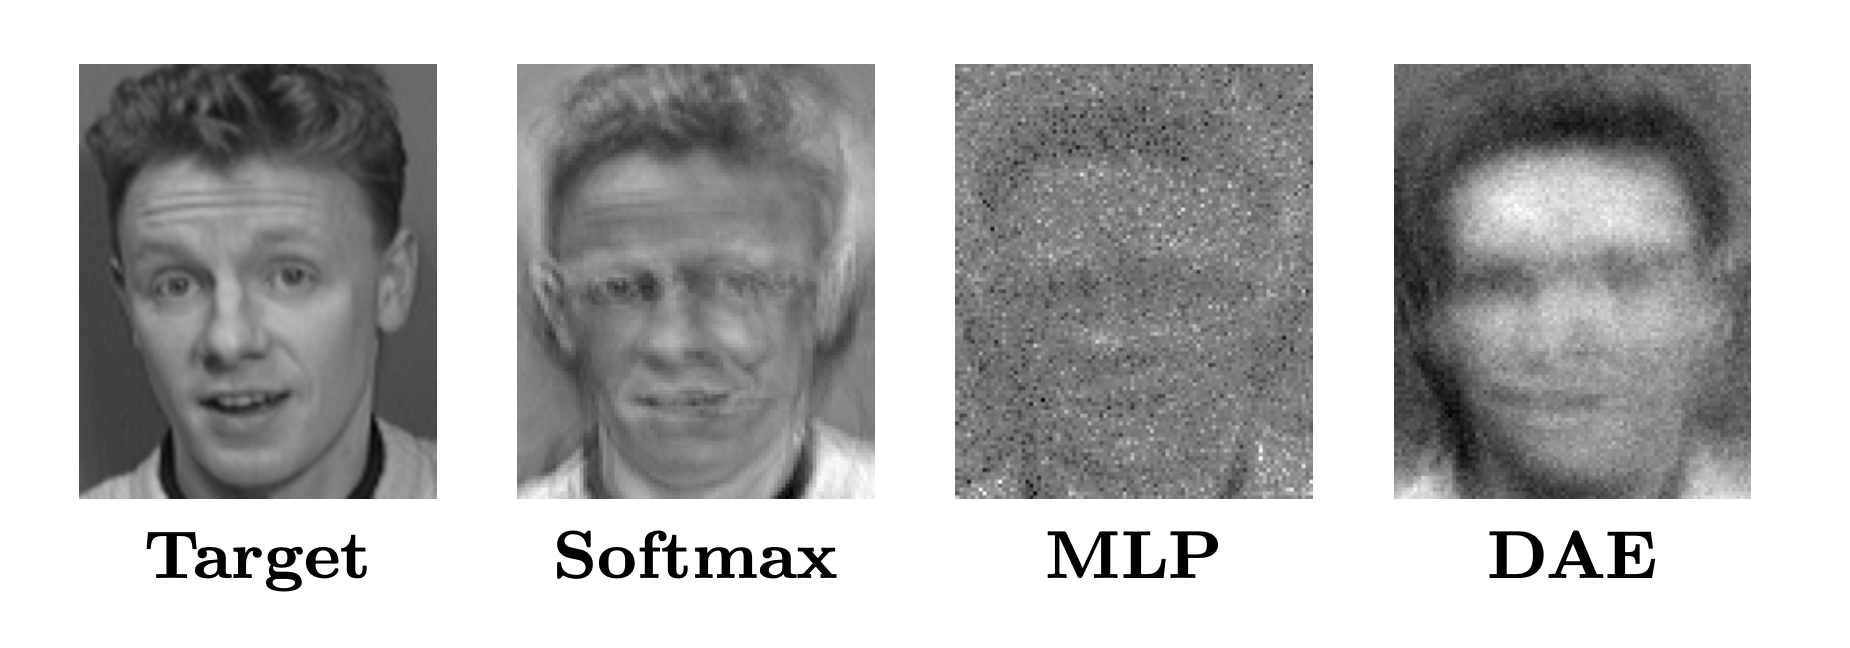
\includegraphics[width=0.8\linewidth]{Bilder/frederikson_2015_3.png}
	\caption{MI-Generierungsqualität der verschiedenen Modelle (\cite[S. 10, Figure 10]{fredrikson_model_2015})}
	\label{img:frederikson_2015_evaluation3}
\end{figure}
Die Genauigkeitsunterschiede zwischen den verschiedenen Durchführungen lässt sich anhand der in Abbildung \ref{img:frederikson_2015_evaluation3} dargestellten Generierungsresultate eindeutig erklären. Bilder, die basierend auf dem Softmax-Regressionsmodell generiert wurden, sind schärfer und deutlicher zu erkennen, als die der anderen beiden Modelle.
\section{Gegenmaßnahmen und Abwehrstrategien}\label{chpt:DefenseMI}
%Vorstellung von Forschungsergebnissen zu Gegenmaßnahmen und Abwehrstrategien gegen Model Inversion Attacks.
Um gegen Angriffe vorzugehen und die Genauigkeit dieser signifikant verschlechtern zu können, nutzt man verschiedene Arten von Verteidigungsstrategien. Diese reichen von Sicherung des Datensatzes durch eine Störung bis hin zur gezielten Veränderung der Modellparameter im Training. 

Die erste Verteidigungsstrategie, die im Folgenden beschrieben wird, zeit das Vorgehen zur Erstellung eines differentiell privaten Datensatzes anhand der im Paper beschriebenen \glqq Methode des privaten projizierten Histogramms\grqq{} (eng.: diffferentially-private histogram) (\cite[9]{fredrikson_privacy_2014}). Dem Autor zufolge sind Methoden zur Privatisierung von Datensätzen unter Entwicklern beliebter, da diese somit mehr Freiheit bei der Modellerstellung ohne die Integration interner Sicherheitsmechanismen haben. Für die Durchführung der Sicherheitsmaßnahme werden die numerischen Attribute des Datensatzes in gleichbreite Bins diskretisiert. Die Bin-Breite berechnet sich durch die im Paper beschriebene Heuristik ($(log(n)/n)^{1/(d+1)}$). Die Erstellung dieser privaten Datensätze basiert auf Parametern, die durch die Autoren innerhalb 100 vollständiger Generierungen bezüglich der Genauigkeit eines Regressionsmodells getestet wurden. Genaueres zu Herleitung genomischer Attribute aus einem privaten Datensatz ist in der Publikation nachzulesen (\cite[9]{fredrikson_privacy_2014}). Neben der Veränderung des zugrunde liegenden Datensatzes bringt Frederikson eine weitere Verteidigungsstrategie ein, in welcher die Privatisierung auf Basis des Modells stattfindet, wodurch in diesem Fall ein privates lineares Regressionsmodell entsteht. Durch das Hinzufügen von Laplace-Rauschen zu den Koeffizienten der Ziel-Funktion wird die lineare Regression gesteuert und die Durchführung von Modell-Inversionsangriffen erschwert.
\section{Bewertung von Modell-Inversions-Angriffen}
%Kritische Bewertung der bisherigen Forschungsergebnisse und Methoden